% This is samplepaper.tex, a sample chapter demonstrating the
% LLNCS macro package for Springer Computer Science proceedings;
% Version 2.20 of 2017/10/04
%
\documentclass[runningheads]{llncs}
%KYR: need to ensure included packages don't interfere with LNCS style
%\usepackage[utf8]{inputenc}
%\usepackage{amsthm, amsmath, amssymb}
\usepackage[T1]{fontenc}
% T1 fonts will be used to generate the final print and online PDFs,
% so please use T1 fonts in your manuscript whenever possible.
% Other font encondings may result in incorrect characters.
%
\usepackage{amsfonts} %mathbb
\usepackage{amsmath} %hdots
\usepackage{amssymb} %blacksquare
\usepackage{mathabx} %vDash
\usepackage{mathrsfs} %mathscr
\usepackage{blkarray} %for blockarray
%\usepackage{textcomp}
%\usepackage{xcolor}
%\usepackage{soul}
%\usepackage{ dsfont }
\usepackage{hyperref}
\usepackage{cancel} %for \cancel
\usepackage{algorithm} %for algorithm environment
\usepackage{algcompatible}
\usepackage[noend]{algpseudocode}
%\usepackage{changepage}%http://ctan.org/pkg/changepage
\usepackage{graphicx} %for includegraphics
\usepackage{tikz}
\usepackage{lscape} %for landscape orientation
%\usepackage{float} %for figures
\usetikzlibrary{shapes.misc, positioning}
\usetikzlibrary{arrows.meta}
\tikzset{>={Latex[width=2mm,length=2mm]}}
\usepackage{caption}
\usepackage{subcaption}
\usepackage{mwe}
\usepackage{fontawesome5}
\usepackage{listings}
\usepackage{xcolor}

%% Save the class definition of \subparagraph
\let\llncssubparagraph\subparagraph
%% Provide a definition to \subparagraph to keep titlesec happy
\let\subparagraph\paragraph
%% Load titlesec
\usepackage[compact]{titlesec}
%% Revert \subparagraph to the llncs definition
\let\subparagraph\llncssubparagraph

% Spacing: left, before, after
\usepackage{titlesec}
\titlespacing*{\section}{0pt}{10pt}{2pt}
\titlespacing*{\subsection}{0pt}{5pt}{2pt}


%% \hypersetup{
%%     colorlinks=true,
%%     linkcolor=blue,
%%     filecolor=magenta,
%%     urlcolor=red,
%%     citecolor=teal
%% }

%LNCS:
% If you use the hyperref package, please uncomment the following line
% to display URLs in blue roman font according to Springer's eBook style:
\renewcommand\UrlFont{\color{blue}\rmfamily}
%for qed:
%% \makeatletter
%% \newcommand{\pushright}[1]{\ifmeasuring@#1\else\omit\hfill$\displaystyle#1$\fi\ignorespaces}
%% \newcommand{\pushleft}[1]{\ifmeasuring@#1\else\omit$\displaystyle#1$\hfill\fi\ignorespaces}
%% \makeatother
%% \makeatletter
%% \newcommand{\specialcell}[1]{\ifmeasuring@#1\else\omit$\displaystyle#1$\ignorespaces\fi}
%% \makeatother


%%%%%%%%%%%%%%%%%%%%%%%%%%%%%%%%%%%%%%%%%%%%%%%%%%%%%%%%
% Spacing Magic
%%%%%%%%%%%%%%%%%%%%%%%%%%%%%%%%%%%%%%%%%%%%%%%%%%%%%%%%
%\usepackage{pslatex} % DON'T REMOVE!  BUYS US HALF A PAGE OR MORE!!!!!
%Use only in case of emergencies: \linespread{0.98} %KYR: make lines spaces .99 instead of 1 to save space
\usepackage{times} %KYR: substitute for pslatex that does not mess up math :)
%\usepackage{savetrees} %KYR: maybe also helps... if we can fix the text to enable this

\usepackage{enumitem}
\setlist[itemize]{noitemsep, nolistsep, topsep=0pt, partopsep={0pt}} 

%CAUTION: dirty trick; questionably allowed... use ONLY in case of emergencies!
% \linespread{0.99}

%%%%%%%%%%%%%%%%%%%%%%%%%%%%%%%%%%%%%%%%%%%%%%%%%%%%%%%%
% Figure Magic
%%%%%%%%%%%%%%%%%%%%%%%%%%%%%%%%%%%%%%%%%%%%%%%%%%%%%%%%
%\usepackage{epsfig}
\usepackage{float} % put figure in minipage
%\usepackage{framed}
%\usepackage{subfigure}

% diagonal line in the table
%\usepackage{diagbox}

% Used in REST experiment section
\usepackage{wrapfig}

\usepackage{enumitem}
\newlist{Properties}{enumerate}{2}
\setlist[Properties]{label=Property \arabic*.,itemindent=*}

%\usepackage{tikz}
%\newcommand*\circled[1]{\tikz[baseline=(char.base)]{
%            \node[shape=circle,draw,inner sep=0.5pt] (char) {#1};}}
%
%\newcommand{\VarPhiSequence}{\ensuremath{\langle T_{\varphi} \rangle}\xspace}
%\newcommand{\ExSeq}[1]{\ensuremath{\langle T_{#1} \rangle}\xspace}
%\newcommand{\ExSeqElement}[2]{\ensuremath{\langle T^{#1}_{#2} \rangle}\xspace}
%\newcommand{\IN}{\mathbb{N}}  

% draw box around text
\usepackage{tcolorbox} 

\renewcommand{\topfraction}{.99} %figures can take up at most 99% of the page before being alone
\renewcommand{\bottomfraction}{.99} %figures can take up at most 99% of the page before being alone
\renewcommand{\textfraction}{.01} %at most this % of page will be text before making figure-only page
\addtolength{\textfloatsep}{-5mm}
\addtolength{\floatsep}{-5mm}
\addtolength{\intextsep}{-5mm}
\addtolength{\abovecaptionskip}{-3mm}
\addtolength{\belowcaptionskip}{-2mm}
\addtolength{\abovedisplayskip}{-5pt}
\addtolength{\belowdisplayskip}{-5pt}


%%%%%%%%%%%%%%%%%%%%%%%%%%%%%%%%%%%%%%%%%%%%%%%%%%%%%%%%
\renewcommand{\phi}{\varphi}


\begin{document}
%
\title{Mission-time Linear Temporal Logic Inference via Structured Grammar Evolution
% \thanks{Iowa State University}
}
%
%\titlerunning{Abbreviated paper title}
% If the paper title is too long for the running head, you can set
% an abbreviated paper title here
%
\author{Zili Wang}
% \author{Zili Wang\inst{1}\orcidID{0000-1111-2222-3333}}
%
\authorrunning{Wang}
% First names are abbreviated in the running head.
% If there are more than two authors, 'et al.' is used.
%
\institute{Iowa State University
\email{ziliw1@iastate.edu}}
%
\maketitle              % typeset the header of the contribution
%
\begin{abstract}
This report examines preliminary work in using Structured Grammar Evolution to tackle the problem of inferring Mission-time Linear Temporal Logic formulas from data.
% \keywords{First keyword  \and Second keyword \and Another keyword.}
\end{abstract}
%
%
%
\section{Introduction}
% \textcolor{red}{FIND RELEVANT PAPERS IN THESE DOMAINS\\}
Learning intuitive high-level temporal properties from the the observed behaviors of complex systems is an important problem that arises in applications such as specification mining for formal verification, debugging systems, behavior classification, and explainable models. 

We focus on the problem of learning, or inferring, Mission-time Linear Temporal Logic (MLTL) properties from observed traces of the system labeled as positive (desirable) or negative (undesirable). The goal is to infer interpretable MLTL classifier over finite traces that can separate the set of positive and negative traces. 

We prove a theoretically interesting results for MLTL: that the class of languages recognized by MLTL classifiers is a strict subset of regular languages. 
Additionally, we propose a novel Grammatical Evolution(GE) algorithm, DSGE$^+$, an implementation of this algorithm, a set of MLTL benchmarks for future research, and experimental evaluation.

\section{Related Work}
There is a large corpus of work on learning regular languages, stemming from Angluin's $L^*$ algorithm \cite{Angluin_1987} that learns a minimal deterministic finite automata (DFA) from positive and negative examples. 

% \textcolor{red}{Expand more on the approaches and challenges people have encountered\\}
Work in learning temporal logic formulae have also recently been explored, and two commonly defined settings are learning from only positive traces, or learning from both positive and negative traces.
Roy et al.\cite{roy_ltlf_learning} proposes two approaches for learning LTL$_f$ from only positive traces. 
The first is a symbolic approach that encodes inference as a constraint satisfaction problem, and the second is a counter-example guided one that generates negative examples in order to guide the learning process. 
Camacho and McIlraith \cite{camacho_ltlf_learning} proposed a symbolic approach to learn LTL$_f$ from positive and negative traces, by using alternating automata to search through a limited space of formula templates.
Further assumption of noisy data motivated Luo et al.\cite{Luo_Liang_Du_Wan_Peng_Zhang_2022} to propose a deep learning approach to extract candidate formulas from graph neural networks trained on positive and negative traces.
In 2018, Nenzi et al. applies evolutionary algorithms to learn Signal Temporal Logic (STL) formulas from (possibly noisy) positive and negative traces. 

The problem of learning Mission-time Linear Temporal(MLTL) Logic has not been explored in the literature. Although MLTL is a more recently introduced fragment of Metric Temporal Logic (MTL), there also are no known related work on learning MTL formulae from example traces. 

\section{Mission-time Linear Temporal Logic}
Mission-time linear temporal logic (MLTL)\cite{Li_Vardi_Rozier_2022} is a finite variation of LTL over bounded, closed, discrete intervals of the form $[a,b]$ where $a,b \in \mathbb{N}$ and $0 \leq a \leq b$. 
The syntax of MLTL formulas, over a finite set of atomic propositions $\mathcal{AP}$, where $p \in \mathcal{AP}$ is a propositional variable, and $\phi$ and $\psi$ are subformulas is as follows: 
$$\phi, \psi := \text{true} \ | \ \text{false} \ | \ p \ | \ \neg \phi \ | \ \phi \land \psi \ | \ \phi \lor \psi \ | \ \mathcal{F}_{[a,b]} \phi \ | \ \mathcal{G}_{[a,b]} \phi \ | \ \phi \mathcal{U}_{[a,b]} \psi \ | \ \phi \mathcal{R}_{[a,b]} \psi.
$$
The symbols $\mathcal{F}, \mathcal{G}, \mathcal{U}, \mathcal{R}$ respectively denote the temporal operators Finally, Globally, Until, and Release. 
MLTL formulas are semantically defined over finite traces bounded by base-10 intervals. A trace $\pi$ of length $|\pi| = m$ is a sequence $\{\pi[i]\}_{i = 0}^{m-1}$ of sets of atomic propositions, $\pi[i] \subseteq \mathcal{AP}$. An atomic proposition $p$ is true at time step $i$ if and only if $p \in \pi[i]$, and the suffix of $\pi$ starting at $i$ (inclusive) is denoted by $\pi_i$, and $\pi_0 = \pi$.
We define that a trace $\pi$ satisfies MLTL formula $\alpha$, denoted $\pi \vDash \alpha$, as follows:\\
\begin{minipage}{0.5\textwidth}
\begin{flalign*}
   &\pi \vDash p \text{ iff } p \in \pi[0]&\\
   &\pi \vDash \alpha \land \beta \text{ iff } \pi \vDash \alpha \text{ and } \pi \vDash \beta&
\end{flalign*}
\end{minipage}
\begin{minipage}{0.5\textwidth}
\begin{flalign*}
    &\pi \vDash \neg \alpha \text{ iff } \pi \nvDash \alpha&\\
    &\pi \vDash \alpha \lor \beta \text{ iff } \pi \vDash \alpha \text{ or } \pi \vDash \beta&
\end{flalign*}
\end{minipage}
% \vspace{-\baselineskip}
\begin{flalign*}
    &\pi \vDash \mathcal{F}_{[a,b]}\alpha \text{ iff } |\pi| > a \text{ and } \exists i \in [a,b] \text{ such that } \pi_i \vDash \alpha&\\
    &\pi \vDash \mathcal{G}_{[a,b]}\alpha \text{ iff } |\pi| \leq a \text{ or } \forall i \in [a,b] \ \pi_i \vDash \alpha&\\
    &\pi \vDash \alpha \ \mathcal{U}_{[a,b]} \beta \text{ iff } |\pi| > a \text{ and } \exists i \in [a,b] \text{ such that } \pi_i \vDash \beta \text{ and }\forall j \in [a, i-1]\ \pi_j \vDash \alpha &\\
    &\pi \vDash \alpha \ \mathcal{R}_{[a,b]} \beta \text{ iff } |\pi| \leq a \text{ or } \forall i \in [a,b] \ \pi_i \vDash \beta \text{ or }\exists j \in [a,b-1] \text{ such that } \pi_j \vDash \alpha &\\
    &\indent \text{ and } \forall a \leq k \leq j \ \pi_k \vDash \beta&
\end{flalign*}
Two formulas $\phi$ and $\psi$ are \textit{semantically} equivalent, denoted $\phi \equiv \psi$, when $\pi \vDash \phi$ if and only if $\pi \vDash \psi$. These semantics preserve the usual operator equivalences in LTL, such as
$\mathcal{F}_{[a, b]} \phi \equiv \text{true } \mathcal{U}_{[a,b]} \phi$,
$\mathcal{G}_{[a, b]} \phi \equiv \text{false } \mathcal{R}_{[a,b]} \phi$, and
$\phi \mathcal{U}_{[a, b]} \psi \equiv \neg (\neg \phi \mathcal{R}_{[a, b]} \neg \psi)$. Note that the neXt ($\mathcal{X}$) operator from LTL$_f$ is semantically equivalent $\mathcal{G}_{[1, 1]}$.

The computation length of a formula $\phi$, denoted $\text{cplen}(\phi)$, is defined in definition $5$ (propagation delay) of \cite{kempa_r2u2}, and can be thought of as the maximum length of a trace that $\phi$ can specify behavior over. 


\subsection{MLTL is Sub-Regular}
A trace $\pi$ with $m$ time steps over $n$ atomic propositions $\mathcal{AP} = \{p_0, ..., p_{n-1}\}$ can be represented as a binary string $w \in \{0, 1\}^*$ of length $mn$. Let $w[i]$ denote the $i$-th bit of $w$ \footnote{We use $0$-indexing in this paper.}, and we may encode $\pi$ by setting $w[n\cdot i +k] = 1$ if and only if $p_k \in \pi[i]$.

\noindent \textbf{Example} For $n=2$ atomic propositions, the word $w = 110100$ specifies a trace over $3$ time steps in which $p_0$ and $p_1$ are both true at time step $0$, only $p_1$ is true at time step $1$, and no atomic propositions are true at time step $2$. Note that we will assume the string representation of computations for the remainder of this paper, and explicitly fix the value of $n$ in all contexts. 

Thus for a MLTL formula $\phi$ over $n$ atomic propositions, we may define \\
$\mathcal{L}(\phi) = \{\pi \in \{0, 1\}^* : |\pi| \equiv 0 (\text{mod }n), \pi \vDash \phi\}$, and also define \\
$L_{MLTL} = \{L \subseteq \{0, 1\}^* : L = \mathcal{L}(\phi) \text{ for some MLTL formula } \phi\}$ as the class of languages recognized by MLTL formulas.

\begin{theorem}
$L_{MLTL}$ $\subsetneq REG$, where $REG$ is the class of regular languages.
\end{theorem}
\begin{proof}
We first prove that $L_{MLTL} \subseteq REG$. 
For any MLTL formula $\phi$, \cite{Elwing_Gamboa-Guzman_Sorkin_Travesset_Wang_Rozier_2024} computes a regular expression $\text{reg}(\phi)$ that captures all traces $\pi$ over $\text{comp\_len}(\phi)$ time steps which satisfy $\phi$. 
Note that this previous work assumes time steps are explicitly separated by commas, while we implicitly separate time steps by fixing $n$ in all contexts. 
Then we have that $\mathcal{L}(\phi) = \mathcal{L}\big(\text{reg}(\phi) (S^n)^*\big)$, where $S$ is shorthand for $(0 | 1)$, which is regular by definition. 

Next, we prove that for any fixed integer $n \geq 1$, no MLTL formula $\phi$ over $n$ propositional variables exists such that $\mathcal{L}(\phi) = L$, where $L = \mathcal{L}\big(S^* 1 \big)$. Suppose for the sake of contradiction that for some fixed integer $n \geq 1$, $\mathcal{L}(\phi) = L$. By the previous argument, we have that $\mathcal{L}(\phi) = \mathcal{L}\big(\text{reg}(\phi) (S^n)^*\big) = \mathcal{L}(\text{reg}(\phi)) \cdot \mathcal{L}(S^*)$, where $\cdot$ denotes the usual concatenation operator between languages. Observe that $\mathcal{L}(\text{reg}(\phi))$ is a finite language containing only strings of length $n\times\text{comp\_len}(\phi)$. If $\mathcal{L}(\text{reg}(\phi)) = S^{n\times\text{comp\_len}(\phi)}$, then $\mathcal{L}(\phi) = S^* \neq L = \mathcal{L}\big(S^* 1 \big)$. Otherwise, there exists $w \notin \mathcal{L}(\text{reg}(\phi))$ such that $|w| = n\times\text{comp\_len}(\phi)$, but then $w\cdot1 \notin \mathcal{L}(\phi)$, while $w\cdot1 \in L = \mathcal{L}\big(S^* 1 \big)$. Thus we conclude that no such $\phi$ may exist, and so $L_{MLTL}$ $\subsetneq REG$.
\end{proof}

\subsection{MLTL Inference is Well-Defined}
We formally define the MLTL inference problem and show that it is well-defined. Fix some integer $n \leq 0$, and let $\Pi^+$ be a set of positive traces, and $\Pi^-$ be a set of negative traces, where $\Pi^+ \cap \Pi^- = \emptyset$. Then the goal is to learn an MLTL formula $\phi$ over $n$ atomic propositions that separates $\Pi = \Pi^+ \cup \Pi^-$, meaning for all $\pi \in \Pi^+$ we have $\pi \vDash \phi$ and for all $\pi \in \Pi^-$ we have $\pi \nvDash \phi$.

\begin{definition}
    An instance of the MLTL inference problem is a triplet $(\Pi^+, \Pi^-, n)$ where $\Pi^+$ and $\Pi^-$ are sets of positive and negative traces, respectively, and $n \geq 1$ is some integer. 
\end{definition}
\begin{theorem}
    For any instance of the MLTL inference problem, $(\Pi^+, \Pi^-, n)$, there exists MLTL formula $\phi$ over $n$ atomic propositions to separate $\Pi = \Pi^+ \cup \Pi^-$. 
\end{theorem}
\begin{proof}
    For any trace $\pi = \pi[0],\pi[1],...,\pi[m]$, we can construct a MLTL formula $\phi_\pi$ such that $\mathcal{L}(\phi_\pi) = \{\pi\}$ by taking  $\phi_\pi = \bigwedge_{i = 0}^{m} G_{[i, i]}(\ell_{i,0} \land ... \land \ell_{i, n-1})$, where $\ell_{i, j} = p_j$ if $p_j \in \pi[i]$, otherwise $\ell_{i, j} = \neg p_j$. 
    % Also note that $\mathcal{L}(\neg \phi_\pi) = \overline{\mathcal{L}(\neg \phi_\pi)}$. 
    Then the formula $\phi = \bigwedge_{\pi \in \Pi^+} \phi_\pi$ 
    % \land \bigwedge_{\pi \in \Pi^-}\neg \phi_\pi$ 
    separates $\Pi$.
\end{proof}

However, this construction of brute force enumeration of all positive traces is only of theoretical interest. In practice, we should strive to learn formulas of size logarithmic with respect to the total size of example traces $\Pi$, i.e. formulas that are good high-level descriptors of $\Pi$. Thus rather than striving for a formula $\phi$ that separates $\Pi$ exactly, we maximize the accuracy of $\phi$ over $\Pi$, defined as 
$$\text{acc}(\phi, \Pi) = 
\frac{|\{\pi \in \Pi^+ : \pi \vDash \phi\}| + |\{\pi \in \Pi^- : \pi \nvDash \phi\}|}{|\Pi|}$$
% \textcolor{red}{\\CAN WE PROVE SOME NICE THEORETICAL RESULT HERE? MAYBE IF STRICT SEPARATION WAS RELAXED TO ($1-\epsilon$) APPROXIMATE SEPARATION?}
\section{Grammar Evolution}
Grammatical Evolution (GE) lie at the intersection of genetic algorithms and formal grammars. As a unique form of genetic programming, GE guides the evolutionary process by translating genetic strings, encoded as chromosomes, into syntactically correct programs or solutions based on a predefined context-free grammar. 

In GE, individual candidate solutions are represented by a collection of genes, which make up the genetic chromosome of the individual. 
Chromosomes are commonly represented as lists of integers, with each integer representing a single gene. 
While genotype refers to the genetic makeup of an individual, an individual's phenotype refers to the expressed characteristics or the solution derived from the genotype. 
In traditional GE, the genotype to phenotype mapping builds a derivation tree by using an individual's genes to select rules from the grammar for expanding nonterminal symbols. 
One important consideration in this mapping process is some way of limiting the maximum depth of a derivation tree, in order to avoid uncontrolled blowup of solution sizes. 

A group of such individuals forms a population in the evolutionary context.
Within this population, each individual is evaluated to determine its fitness, which is a measure of how well the phenotype solves the problem at hand. 
This evaluation critically guides the selection process, during which individuals are chosen for reproduction based on their fitness levels. The selection process, often inspired by natural selection, favors individuals with higher fitness while allowing some degree of randomness to maintain population diversity.

Following selection, crossover and mutation operators generate a new generation of individuals. 
Crossover exchanges segments of chromosomes between pairs of individuals, resulting in offspring with genetic traits inherited from both parents. 
Mutation introduces random alterations to an individual's genes, which helps maintain genetic diversity within the population. 
These processes are crucially explore new regions of the solution space prevents the population from converging prematurely. 

Lastly, the new generation of individuals then replaces some or all of the existing population in a step known as replacement. 
This could be done through various strategies, such as removing the least fit individuals or adopting an elitist approach where the best-performing individuals are retained. 
Through these iterative cycles of selection, crossover, mutation, and replacement, the population evolves over successive generations, ideally moving towards increasingly effective solutions.

GE is commonly criticized for its lack of locality and high redundancy. 
In \cite{Rothlauf_Oetzel_2006}, Rothlauf and Oetzel demonstrated that over 90\% of changes to a particular gene in the genotype do not affect the phenotype.
In the remaining 10\% of cases, the change to the phenotype is often drastic, and two individuals with nearly identical genotypes may have very different phenotypes.
These issues impede the search process, as the crossover and mutation operators essentially simulate a random walk in the solution space.

\subsection{GE Variants}
\subsubsection{Structured Grammatical Evolution} (SGE) \cite{lourenco_sge_2016} is a variant of GE that attempts to address the issues of locality and redundancy.
In SGE, genotypes are a list of list of integers, where each nonterminal symbol in the grammar is associated with a list of integers.
SGE limits the maximum depth of a derivation tree by introducing indexed copies of each recursive nonterminal, which can be expensive depending on grammar structure.

The genotype to phenotype mapping in SGE builds a derivation tree by using an individual's genes to select rules from the grammar for expanding nonterminal symbols.
This extra structure imposed by SGE ensures that modification of a single gene affects only the corresponding nonterminal symbol in the phenotype. 

\subsubsection{Dynamic Structured Grammatical Evolution} (DSGE) \cite{lourenco_sge_2016} introduced by Lourenco et al. addresses the issue of grammar preprocessing in SGE.
The genotype to phenotype mapping takes a maximum depth parameter and upon reaching maximum depth, the \texttt{generate\_terminal\_expansion} function maps a recursive nonterminal to a non-recursive nonterminal or a terminal.

In DSGE, genotypes encode only genes that are expressed in the phenotype (the parse tree) of the individual. 
During evolution, changes to the genotype gives rise to instances where new integers may need to be added to a gene array that ``runs out'' of genes. 
As a result of the dynamic nature of the genotype, the initialization procedure requires first building a derivation tree from the grammar and then encoding the tree into a genotype. 
In contrast, GE and SGE initialize individuals by mapping randomly generated genotypes to phenotypes. 

\section{DSGE$^+$ for MLTL} 
We propose DSGE$^+$ as a variant of DSGE that addresses the unnecessary complexity of the initialization procedure as well as the phenomenon of individuals ``running out'' of genes during evolution.
We proceed to describe the details of DSGE$^+$ in the context of a specific MLTL grammar.

\subsection{MLTL Grammar}
A common challenge in all applications of GE is a good grammar representation of the solution space. 
Such a grammar should capture certain structural properties of the problem domain, and we use a grammar that is defined dynamically based on the example traces. 
Let $(\Pi^+, \Pi^-, n)$, where $\Pi = \Pi^+ \cup \Pi^-$ be an instance of the MLTL inference problem, and we define the length of the longest trace as $m = \max_{\pi \in \Pi} |\pi|$. 
Then we only need to consider variables $p_0, ..., p_{n-1}$ and intervals of the form $[a, b]$ for $0 \leq a \leq b \leq m$.
We define the MLTL grammar as follows:

\begin{align*}
    \langle \text{wff} \rangle ::={} & \langle \text{prop\_cons} \rangle \\
    \mid & \langle \text{prop\_var} \rangle \\
    \mid & \lnot \langle \text{wff} \rangle \\
    \mid & ( \langle \text{wff} \rangle \, \langle \text{binary\_prop\_conn} \rangle \, \langle \text{wff} \rangle ) \\
    \mid & \langle \text{unary\_temp\_conn} \rangle \, \langle \text{interval} \rangle \, \langle \text{wff} \rangle \\
    \mid & ( \langle \text{wff} \rangle \, \langle \text{binary\_temp\_conn} \rangle \, \langle \text{interval} \rangle \, \langle \text{wff} \rangle ) \\
    \langle \text{binary\_prop\_conn} \rangle ::={} & \land \mid \lor \mid \rightarrow \\
    \langle \text{unary\_temp\_conn} \rangle ::={} & F \mid G \\
\end{align*}
\begin{align*}
    \langle \text{binary\_temp\_conn} \rangle ::={} & U \mid R \\
    \langle \text{interval} \rangle ::={} & [a, b] \quad \text{for } 0 \leq a \leq b \leq m \\
    \langle \text{prop\_cons} \rangle ::={} & \text{true} \mid \text{false} \\
    \langle \text{prop\_var} \rangle ::={} & p_i \quad \text{for } 0 \leq i < n
\end{align*}
This grammar has $7$ nonterminals symbols, denoted by $\langle \cdot \rangle$. 
Notably, $\langle \text{wff} \rangle$ captures the previously defined syntax of MLTL, and is the only recursive nonterminal. 
The overall structure of this grammar would be very similar to that of other popular temporal logics such as Linear Temporal Logic over finite traces, Metric Temporal Logic, Signal Temporal Logic, Computation Tree Logic, etc. 

\subsection{Genotype to Phenotype Mapping}
We define the branching factor of a grammar as the maximum number of recursive nonterminal symbols in any right-hand-side term of a rule of the form $lhs \rightarrow rhs$. In the MLTL grammar, the branching factor is $2$ because of the two rules for binary temporal connectives and binary propositional connectives.

For a fixed branching factor $b$ and maximum recursion depth $d$, we may calculate that at most $\frac{b^d - 1}{b - 1}$ genes will be expressed from each nonterminal genome.
For $b = 2$, we bound the number of genes expressed from each nonterminal genome by $2^d-1$.

Then the genotype to phenotype mapping is described by algorithm \ref{genomoToPhenome}. 
A direct consequence of this mapping is that the list of popped genes for each nonterminal keeps track of the number of genes that have been expressed. 
This approach enables us to benefit from the advantages of DSGE over GE, specifically in terms of locality and redundancy, as well as DSGE's advantages over SGE in bypassing grammar preprocessing. 
Additionally, it prevents the issue of individuals "running out" of genes during the evolution process and avoids the complexity of the initialization procedure.
Specifically, an individual $x$ may be initialized with a random integer array of length $2^d-1$ for each nonterminal in the grammar. 

\begin{algorithm}
\caption{Initialize Parse Tree from Genotype}
\begin{algorithmic}[1]
\label{genomoToPhenome}
\Procedure{InitializeParseTree}{genotype, grammar}
    \State $tree \gets \text{CreateEmptyTree()}$
    \State $root \gets \text{CreateNode}(\text{"<wff>"})$
    \State $tree.\text{AddRoot}(root)$
    \State $stack \gets \text{new Stack()}$
    \State $stack.\text{push}((root, 0))$ \Comment{Stack of (node, depth)}
    \State $poppedGenes \gets \emptyset$
    \While{$\neg stack.\text{isEmpty}()$}
        \State $(node, depth) \gets stack.\text{pop}()$
        \If{$depth \geq \text{MaxTreeDepth}$ and $\text{IsNonTerminal}(node)$}
            \State $\text{ExpandTerminal}(node, genotype, poppedGenes)$
        \ElsIf{$\text{IsNonTerminal}(node)$}
            \State $\text{ExpandNonTerminal}(node, genotype, grammar, stack, depth, poppedGenes)$
        \EndIf
    \EndWhile
    \State $\text{UpdateGenotype}(genotype, poppedGenes)$
    \State \Return $tree$
\EndProcedure
\end{algorithmic}
\end{algorithm}

\subsection{Genetic Algorithm}
We now proceed to describe the genetic algorithm used to evolve the population of individuals. Let $\Pi = \Pi^+ \cup \Pi^-$ be the set of example traces, $m = \max_{\pi \in \Pi} |\pi|$ be the length of the longest trace, and fix $n \leq 1$ to be the number of atomic propositions.

\subsubsection{Fitness} of an individual with phenotype $\phi$ is defined as:
$$\text{fitness}(\phi) = 
w_1 \cdot \text{acc}(\phi, \Pi) + 
w_2 \cdot \frac{|\text{comp\_len}(\phi)-m|}{m} + 
w_3 \cdot \frac{1}{|\phi|} + 
w_4 \cdot \frac{1}{\text{depth}(\phi)}$$
where $\text{acc}(\phi, \Pi)$ is the accuracy of $\phi$ over $\Pi$, $\text{comp\_len}(\phi)$ is the computation length of $\phi$, $\text{depth}(\phi)$ is the depth of the parse tree of $\phi$, and $w_1, w_2, w_3, w_4$ are hyperparameters that we may tune to emphasize certain properties of the formula.

Achieving high accuracy is the primary goal of the MLTL inference problem, and so we set $w_1 = 0.8$. 
The second term of the fitness function measures the absolute deviation between the computation length of $\phi$ and the length of the longest trace in $\Pi$. 
This term encourages the formula to encode a specification appropriate to observed traces in $\Pi$, and we set $w_2 = 0.1$.
The third term of the fitness function measures the inverse of the length of the formula, defined simply as the number of characters in the formula.
This encourages the formula to be concise and therefore interpretable, and we set $w_3 = 0.04$.  
The fourth term of the fitness function measures the inverse of the depth of the parse tree of $\phi$.
Again, this encourages the formula to be concise and interpretable, and we set $w_4 = 0.01$.
Each of the four terms of the fitness function are normalized to be in the range $[0, 1]$, and so the overall fitness is also in the range $[0, 1]$.

\subsubsection{Selection}
is currently done at each iteration by simply selecting the top $20\%$ of the population based on fitness. 

However, I wish to explore the effect of the a genetic difference operator that measures the genetic difference between two individuals $x$ and $y$. 
Suppose that $A$ is some nonterminal in the grammar, and $x_A$ and $y_A$ are the expressed genomes, represented as a list of integers, of $x$ and $y$ for nonterminal $A$. 
Then define the genetic difference \footnote{It would be cool to prove that this is actually a well-defined distance function satisfying the triangle inequality. At which point the space of solutions forms a metric space and we can look to formalize some aspects of GE with real analysis and topology.}
between $x_A$ and $y_A$ as:
$$
\text{diff}(x_A, y_A) =
\sum_{j = 0}^{\text{max}(|x_A|, |x_B|)-1}
1_{\{x_A[j] \neq y_A[j]\}} \cdot r^j
$$
and the genetic difference between $x$ and $y$ as:
$$
\text{diff}(x, y) =
\sum_{A \in \text{nonterminals}}
w_A \cdot \text{diff}(x_A, y_A)
$$
where $1_{\text{condition}}$ is the indicator function that evaluates to $1$ if the condition is true, and $0$ otherwise, and $w_A$ is a tunable hyperparameter that we use to emphasize the importance of $A$ in the grammar.

To ensure normalization of the genetic difference in the interval $[0, 1]$, we can find the condition on $r$ such that $\text{diff}(x, y) \leq 1$ for all $x, y$:
\begin{align*}
    \text{diff}(x, y) &= \sum_{A \in \text{nonterminals}} w_A \cdot \sum_{j = 0}^{\text{max}(|x_A|, |x_B|)-1}
    1_{\{x_A[j] \neq y_A[j]\}} \cdot r^j\\
    &\leq \sum_{A \in \text{nonterminals}}
    w_A \cdot \sum_{j = 0}^{\infty} r^j\\
    &= \sum_{A \in \text{nonterminals}} w_A \cdot \frac{r}{r-1} \\
    &\leq 1, \text{ implying that } r \geq \frac{1}{1 + \sum_{A \in \text{nonterminals}} w_A}.
\end{align*}

The motivation for the exponential factor $r^j$ is to emphasize the importance of the first few genes in the genome, and to de-emphasize the importance of the later genes. 
For instance, in the context of our MLTL grammar, the first few genes of the $\langle \text{wff} \rangle$ genome are more important than the later genes because the first few genes determine overall structure of the formula. 
Having tunable weights $w_A$ allows us to emphasize certain importance of certain nonterminals determining the structure of the solution. 
We set $w_A = 1$ for all $A \in \text{nonterminals}$ for now, but we may wish to emphasize the importance of $\langle \text{wff} \rangle$ in the future.

This genetic difference operator can be used to perform $k$-clustering on the population, where $k$ is the number of groups we wish to cluster the population into.
We can then perform selection by selecting the top individuals from each cluster, thereby maintaining population diversity without sacrificing the quality of the population.

\subsubsection{Crossover} is done with the standard one-point crossover operation. 
Crossover between two genomes $x_A$ and $y_A$ is done by selecting a random index $i$ and swapping the suffixes of $x_A$ and $y_A$ starting at index $i$.
$i$ is chosen so that it is always at index before the last expressed gene of $x_A$ and $y_A$, and so that the resulting genome always guarantees an individual inherits phenotype attributes from both parents. 

\subsubsection{Mutation} is done with the standard point mutation operation. 
Mutation of a genome $x_A$ simply mutates each gene of $x_A$ with probability $p$. 
At each iteration, we apply an exponential decay factor of $0.95$ to $p$ to encourage early exploration of the solution space and later exploitation of the solution space.

\section{Experimental Evaluation}
Due to the lack of existing MLTL inference benchmarks, we propose a set of benchmarks for future research.
We report and analyze the performance of DSGE$^+$ on these benchmarks. 
For relatively easy benchmarks, we use a population size of $100$ and run the genetic algorithm for $30$ generations, while for more difficult benchmarks, we use a population size of $300$ to $1000$ and run the genetic algorithm for $50$ generations.

One achievement to highlight is the improvement of the efficiency of computing an individual's accuracy score over a set of traces.
This single computation is the bottleneck of the entire algorithm, and significant effort was spent on optimizing this computation.
Originally, the WEST tool \cite{Elwing_Gamboa-Guzman_Sorkin_Travesset_Wang_Rozier_2024} provides a Python implementation of the MLTL semantics, that on inputs MLTL formula $\phi$ and trace $\pi$, returns whether $\pi \vDash \phi$. 
I reimplemented this functionality in C++ and achieved a significant (maybe I should quantify this) speedup.
Further optimizations on batched computation over a set of traces, rather than computing the accuracy score of an individual over each trace individually, resulted in a $20$ times speedup. 
Lastly, parallelizing the computation for each population member over multiple threads resulted in another $3$ times speedup. In total, these optimizations resulted in a $60$ times speedup from initial implementation to final implementation.

\subsection{Benchmarks}
We generate benchmarks by first choosing a target formula $\phi$, and then generating a set of positive traces and negative traces $\Pi = \Pi^+ \cup \Pi^-$. 
Since the WEST tool \cite{Elwing_Gamboa-Guzman_Sorkin_Travesset_Wang_Rozier_2024} gives a regular expression for all traces satisfying $\phi$, we can generate positive traces by randomly sampling the regular expressions. 
Likewise, we can sample negative traces by running WEST on $\neg \phi$. 
However, WEST was not intended for the purpose of solving all-SAT for MLTL, and times out on some of the more difficult benchmarks.
In these cases, we may default to randomly sampling traces to populate $\Pi^+$ and $\Pi^-$.

In total, we created $9$ benchmarks, with $4$ benchmarks that target the basic temporal operators, and $5$ benchmarks that use MLTL formulae found in the literature. For each benchmark, we produced a total of $500$ positive traces and $500$ negative traces. $100$ positive traces and $100$ negative traces were used for training, and the remaining $400$ traces were held out for testing.

\subsubsection{Basic Temporal Operators} targets the basic temporal operators $\mathcal{F}, \mathcal{G}, \mathcal{U}, \mathcal{R}$. The target formulae are:
\begin{enumerate}
    % F[0,10](p0 | p1)
    \item $\mathcal{F}_{[0, 10]} (p_0 \lor p_1)$
    % G[0,10](p0 & (p1 & !p2))
    \item $\mathcal{G}_{[0, 10]} (p_0 \land (p_1 \land \neg p_2))$
    % (p0 R[0,10] p1)
    \item $(p_0 \ \mathcal{R}_{[0, 10]} \ p_1)$
    % (p0 U[0,10] p1)
    \item $(p_0 \ \mathcal{U}_{[0, 10]} \ p_1)$
\end{enumerate}

\subsubsection{DragonEye UAS} was studied by Moosbrugger et al. \cite{Moosbrugger_Rozier_Schumann_2017} using the R2U2 tool. 
R2U2 is a framework for runtime monitoring of system health in Unmanned Aerial Systems (UAS). Several formulas we used from the case study are: 
\begin{enumerate}
    % G[0,10]!(!a0 & !(a1 U[0,10] a0))
    \item $\mathcal{G}_{[0, 10]} \neg (\neg p_0 \land \neg (p_1 \ \mathcal{U}_{[0, 10]} \ p_0))$
    % G[0,65525]!(a6 & !(((!a2 & !a3) & !a4) U[0,65525] a5))
    \item $\mathcal{G}_{[0, 65525]} \neg (p_6 \land \neg (((\neg p_2 \land \neg p_3) \land \neg p_4) \ \mathcal{U}_{[0, 65525]} \ p_5))$
    % G[0,300]((a4 & a5) & a6)
    \item $\mathcal{G}_{[0, 300]} ((p_4 \land p_5) \land p_6)$
\end{enumerate} 
Note that formulas $2$ and $3$ had unfeasibly long computation lengths for the purposes of a genetic algorithm, and so we scaled the computations lengths down to $20$. 

\subsubsection{NASA's NextGen Air Traffic Control} is a air traffic management system that was evaluated by Gario et al. \cite{Gario_Cimatti_Mattarei_Tonetta_Rozier_2016}. 
They came up with $1620$ most relevant designs, and we used $2$ MLTL formulas from their case study as benchmarks. The target formulae are:
\begin{enumerate}
    %((!((a1)&(!(G[505,713]((G[100,100]((true)U[201,979](a0)))&(G[0,287]((true)U[431,483](!(a0)))))))))&(true))
    \item $\neg ((p_1 \land \neg (\mathcal{G}_{[505, 713]} ((\mathcal{G}_{[100, 100]} (\text{true} \ \mathcal{U}_{[201, 979]} \ p_0)) \land (\mathcal{G}_{[0, 287]} (\text{true} \ \mathcal{U}_{[431, 483]} \neg p_0)))) \land \text{true})$
    %((G[369,504]((G[0,34](!((a0)&(!(G[605,1000](a0))))))&(G[496,496](!((a0)&(!((true)U[887,1000](!(a0)))))))))&(true))
    \item $(\mathcal{G}_{[369, 504]} ((\mathcal{G}_{[0, 34]} (\neg (p_0 \land \neg (\mathcal{G}_{[605, 1000]} p_0)))) \land (\mathcal{G}_{[496, 496]} (\neg (p_0 \land \neg (\neg (\text{true} \ \mathcal{U}_{[887, 1000]} \neg p_0)))))) \land \text{true})$
\end{enumerate}
Again, we scaled the computation lengths down to $20$ for the purposes of a genetic algorithm.

\subsection{Results}
We now report and analyze the performance of DSGE$^+$ on each of the benchmarks.
For each benchmark, we track the fitness score, accuracy, computation length, formula length, parse tree depth, and phenotype of the best individual in the population at each generation.

Across all benchmarks, we observe that the fitness score of the best individual in the population increases monotonically over time, by design of the genetic algorithm.
On all of the basic temporal operator benchmarks and formula $3$ of the DragonEye UAS benchmark, a test accuracy of $100\%$ is achieved. 
It's interesting to note that a majority of the time, test accuracy is strictly lower than training accuracy, which is likely due to overfitting.
Additionally, if the training set does not contain an informative trace that the test set contains, then no algorithm can guarantee $100\%$ accuracy on the test set.
For intance in the Until benchmark, the language of the best individual is $\mathcal{L}(\mathcal{F}_{[1, 10]} p_1)$, which is a strict subset of the language of the target formula $\mathcal{L}(\mathcal{F}_{[0, 10]} (p_0 \lor p_1))$. 
This is because the training set does not contain an informative trace in the difference of these languages. 
Such a trace would require $p_1$ to hold at some time step, and then $p_0$ to never hold for the next $10$ time steps, which is a very specific trace that is unlikely to be sampled randomly.

For the more difficult benchmarks, formulae $1$ and $2$ of the DragonEye UAS benchmark, and formulae $1$ and $2$ of the NASA's NextGen Air Traffic Control benchmark, we observe that formula length and parse tree depth first increase, then decrease. 
This trend is due to the high weight given to the formula accuracy, and thus the genetic algorithm prioritizes improving the accuracy first, and then improving the formula length and parse tree depth after the accuracy can not be easily improved.

Another notable trend is that the computation length of the best individual often hovers around $m$, the target computation length.
This behavior is expected and desirable, as the genetic algorithm is incentivized to produce a formula that is appropriate for the observed traces in $\Pi$.

Lastly, we observe that the genetic algorithm is able to learn formulae that are more concise than the target formulae.
For instance, the learned formula in formula $2$ of the DragonEye UAS benchmark, and formulae $1$ and $2$ of the NASA's NextGen Air Traffic Control benchmark, are all more concise than the target formulae.
However, the accuracy of these learned formulae are not $100\%$. 
This suggests that the learned formulae may be a good approximation of the target formulae, and could be a good starting point for rewriting the target formulae into a more concise formula.

\begin{figure}
    \centering
    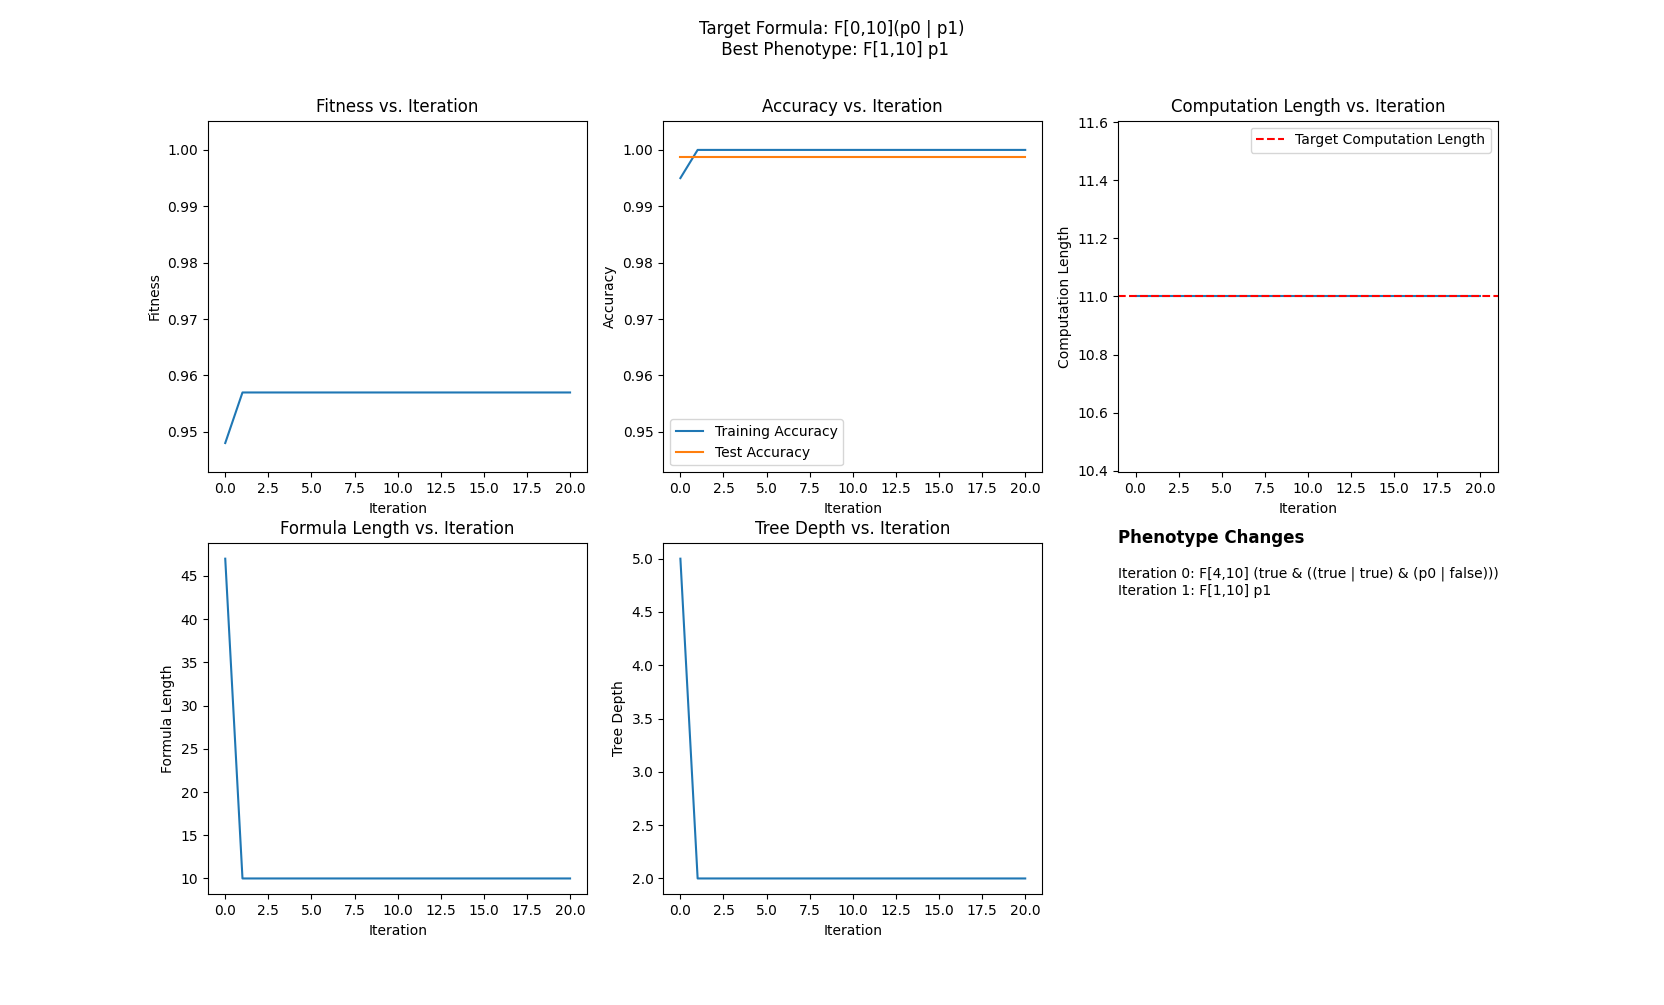
\includegraphics[width=1.1\textwidth]{figs/log_future.txt.png}
    \caption{Training plots of $DSGE^+$ on the future time operator benchmark.}
    \label{fig:future}
\end{figure}

\begin{figure}
    \centering
    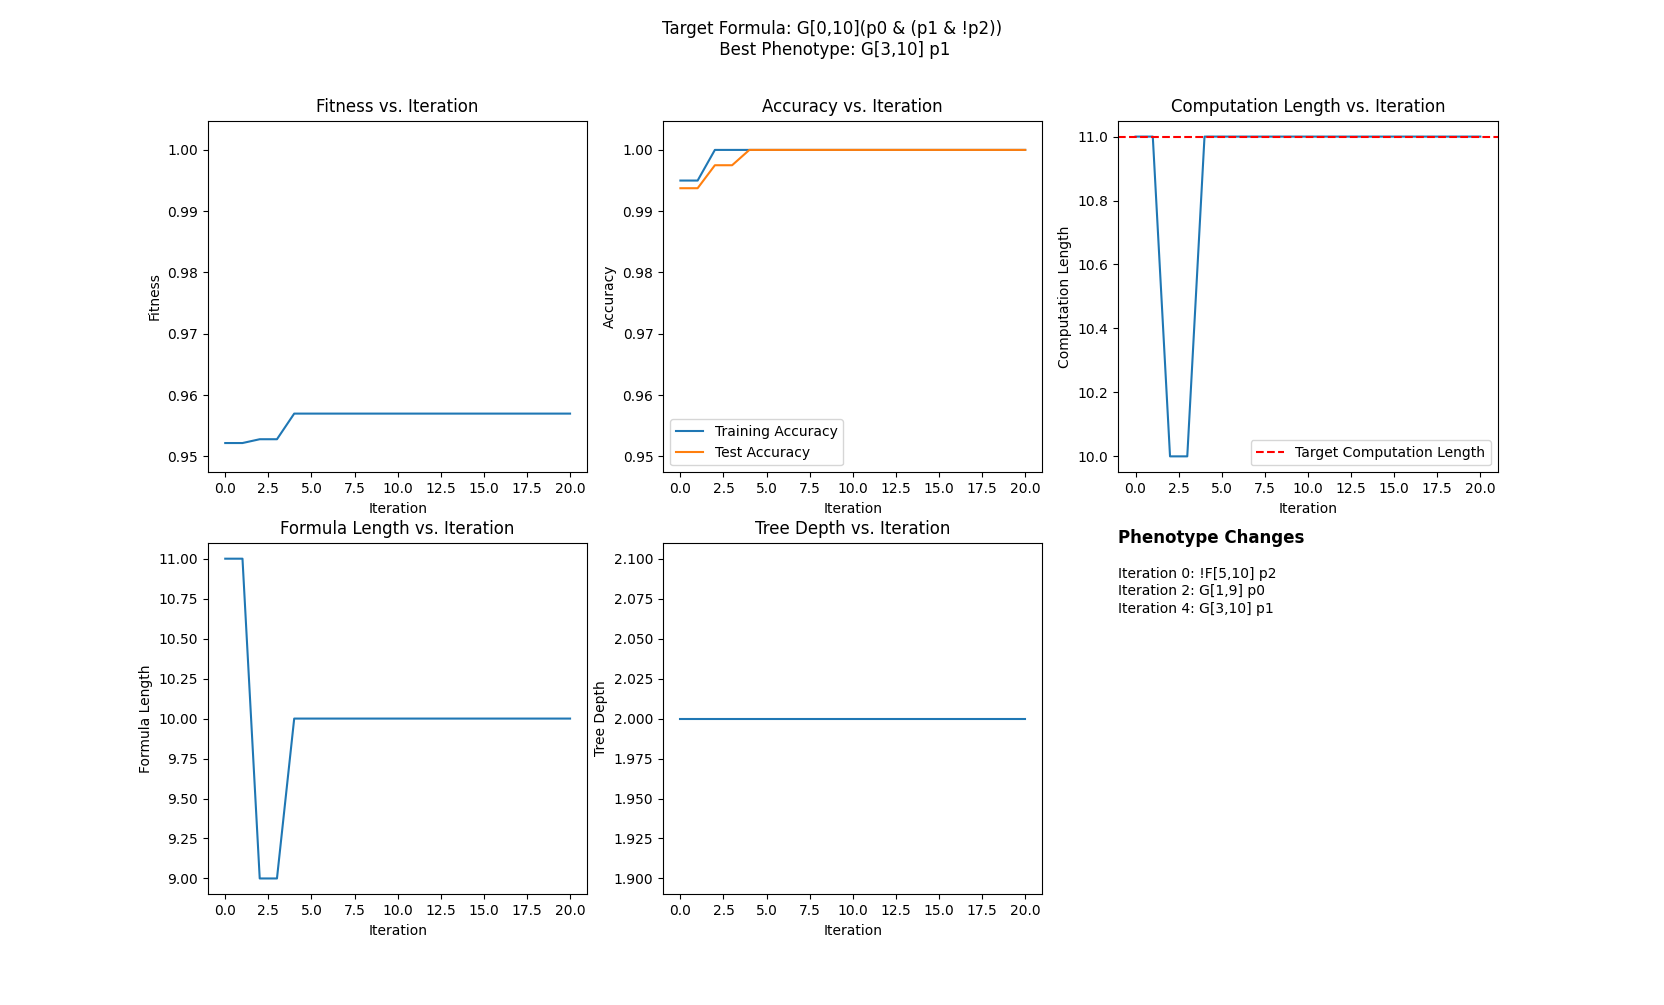
\includegraphics[width=1.1\textwidth]{figs/log_global.txt.png}
    \caption{Training plots of $DSGE^+$ on the globally operator benchmark.}
    \label{fig:global}
\end{figure}

\begin{figure}
    \centering
    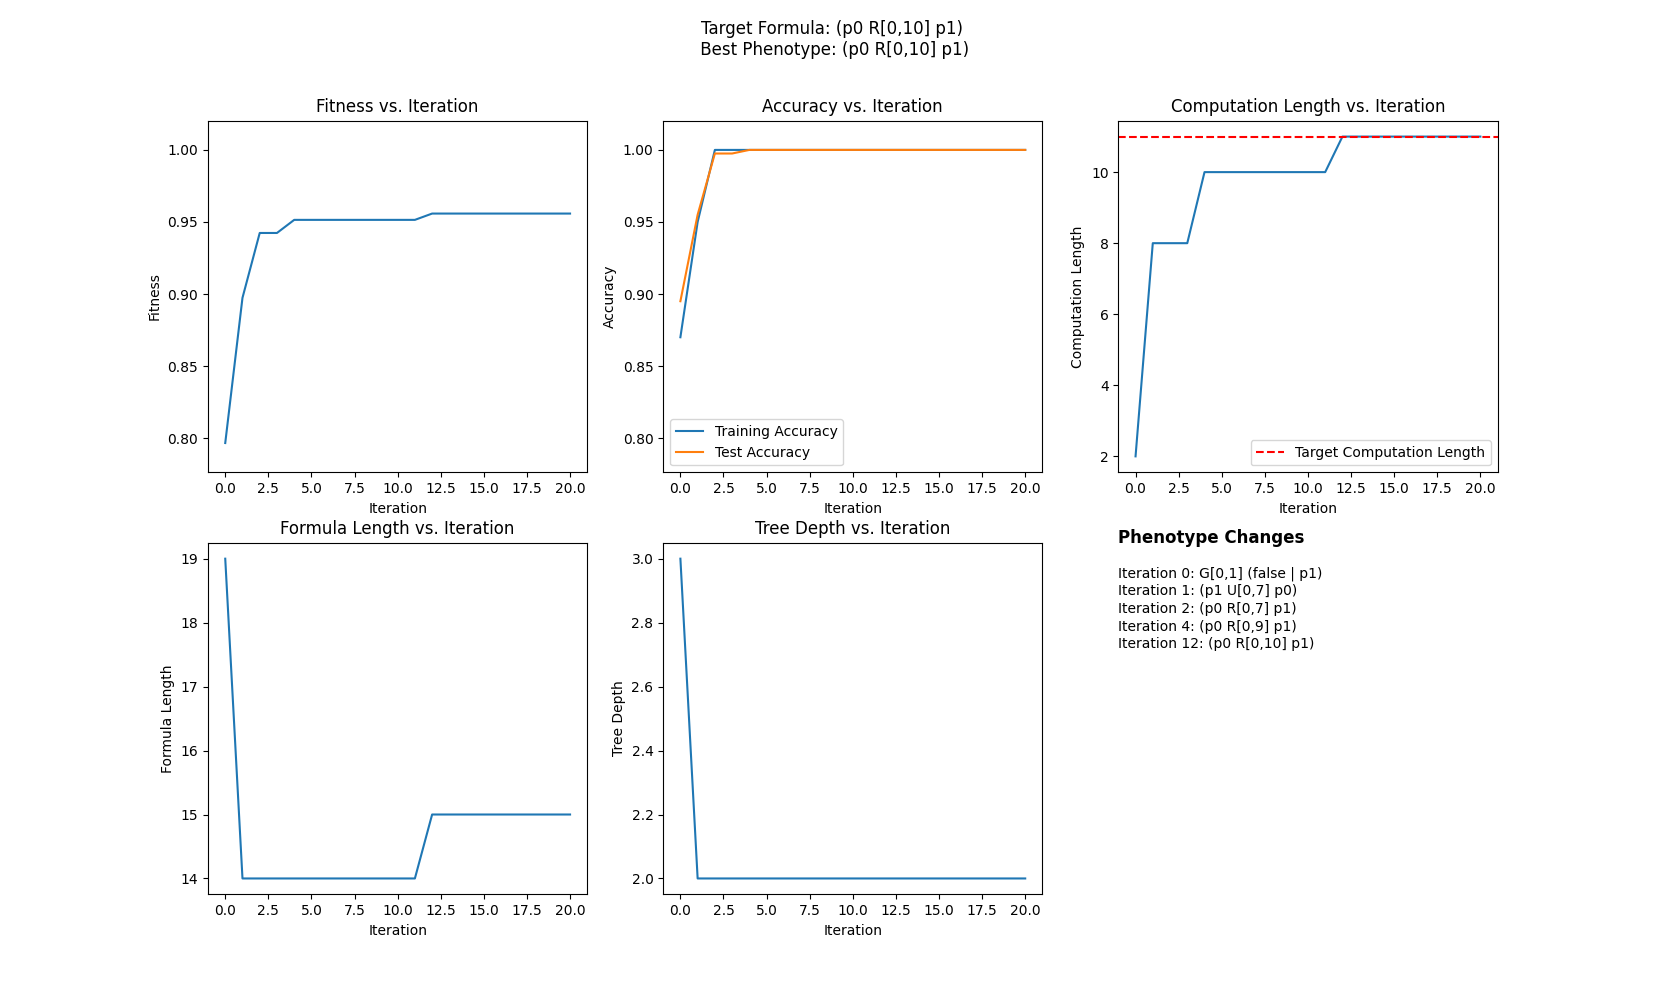
\includegraphics[width=1.1\textwidth]{figs/log_release.txt.png}
    \caption{Training plots of $DSGE^+$ on the release operator benchmark.}
    \label{fig:release}   
\end{figure}


\begin{figure}
    \centering
    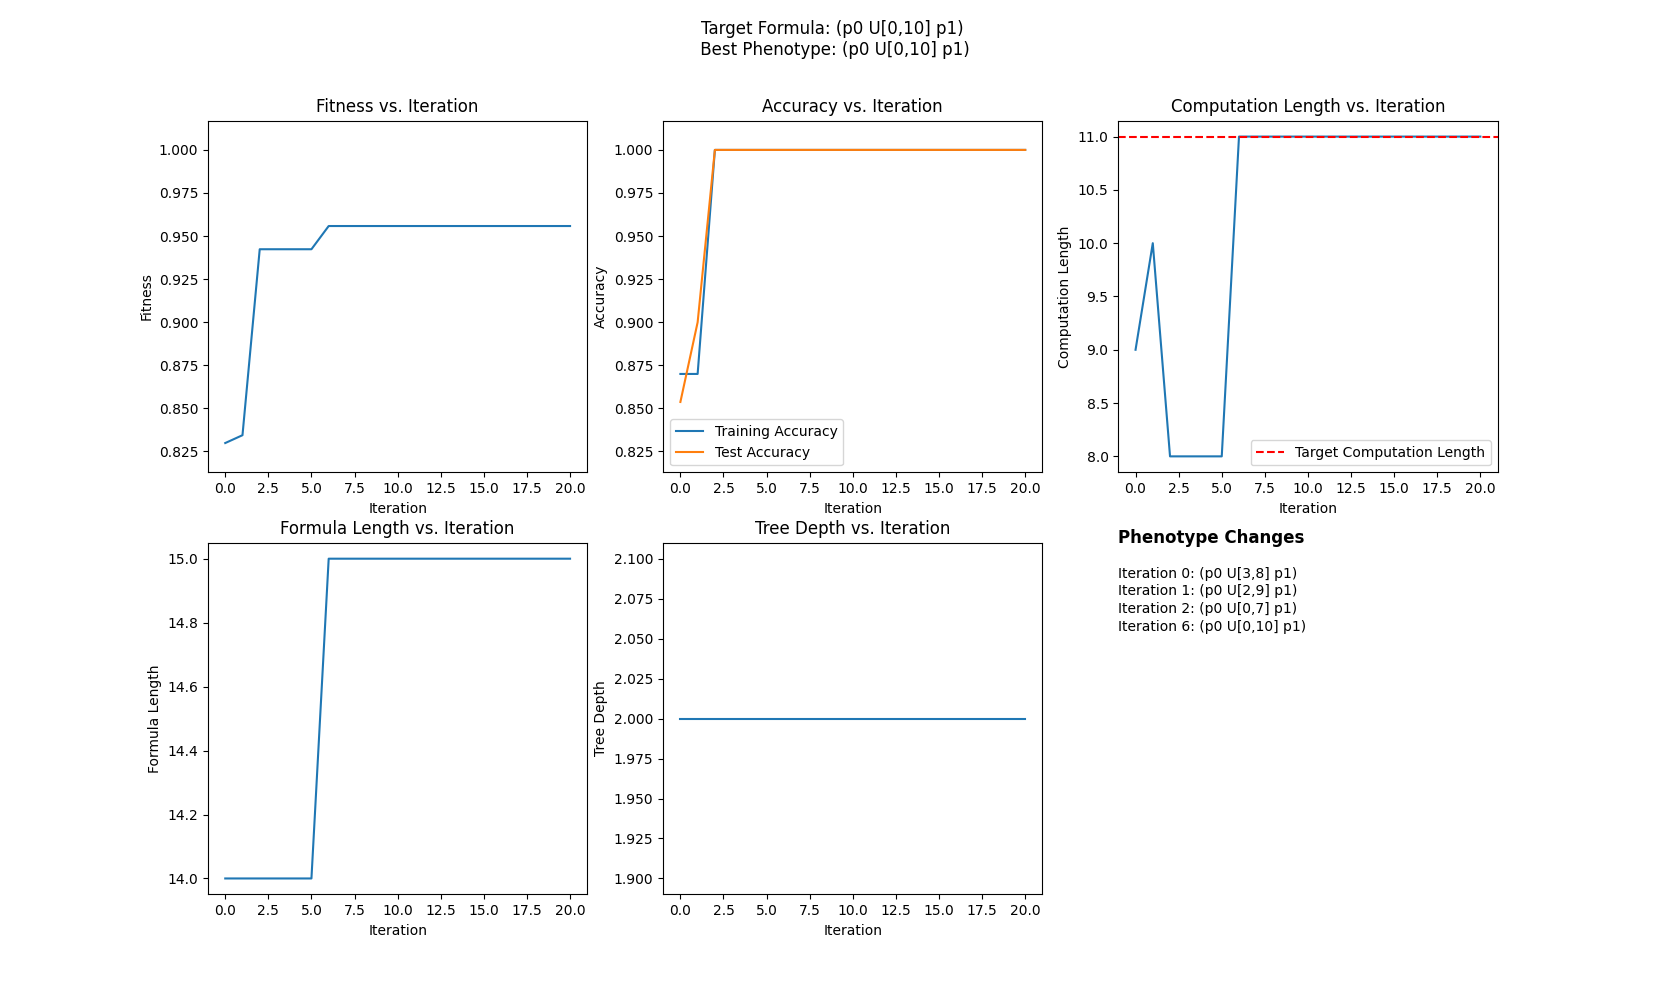
\includegraphics[width=1.1\textwidth]{figs/log_until.txt.png}
    \caption{Training plots of $DSGE^+$ on the until operator benchmark.}
    \label{fig:until}
\end{figure}

\begin{figure}
    \centering
    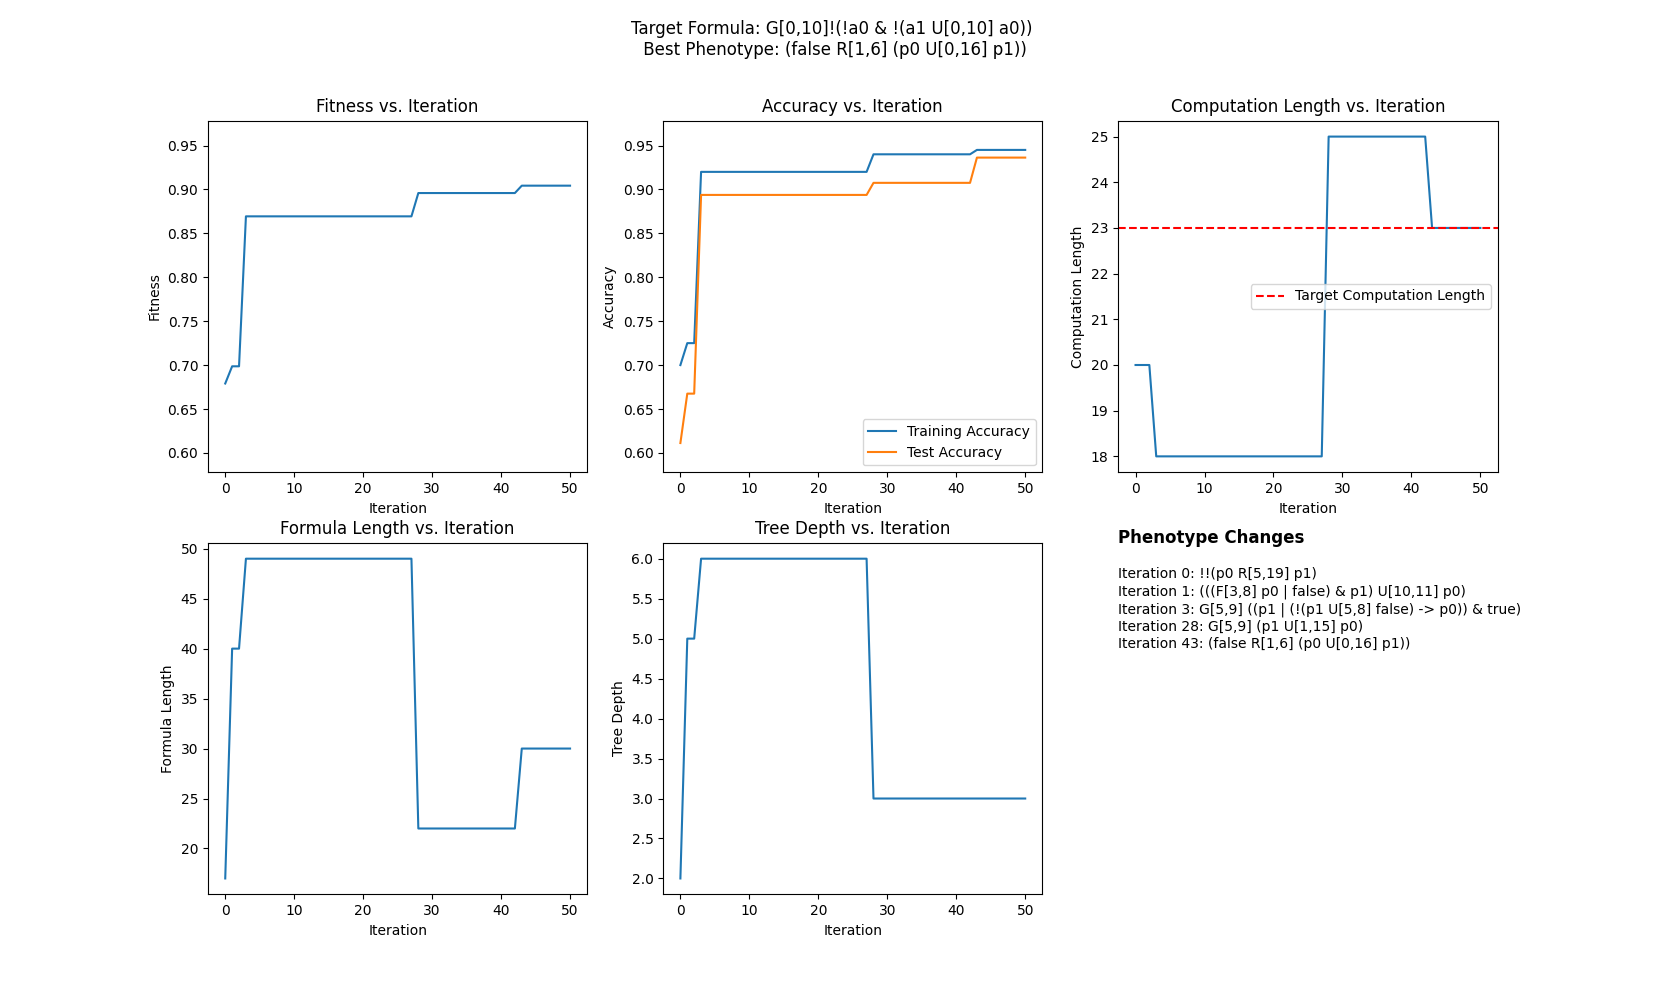
\includegraphics[width=1.1\textwidth]{figs/log_fmsd17_formula1.txt.png}
    \caption{Training plots of $DSGE^+$ formula 1 of the DragonEye UAS benchmark.}
    \label{fig:fmsd17_formula1} 
\end{figure}   

\begin{figure}
    \centering
    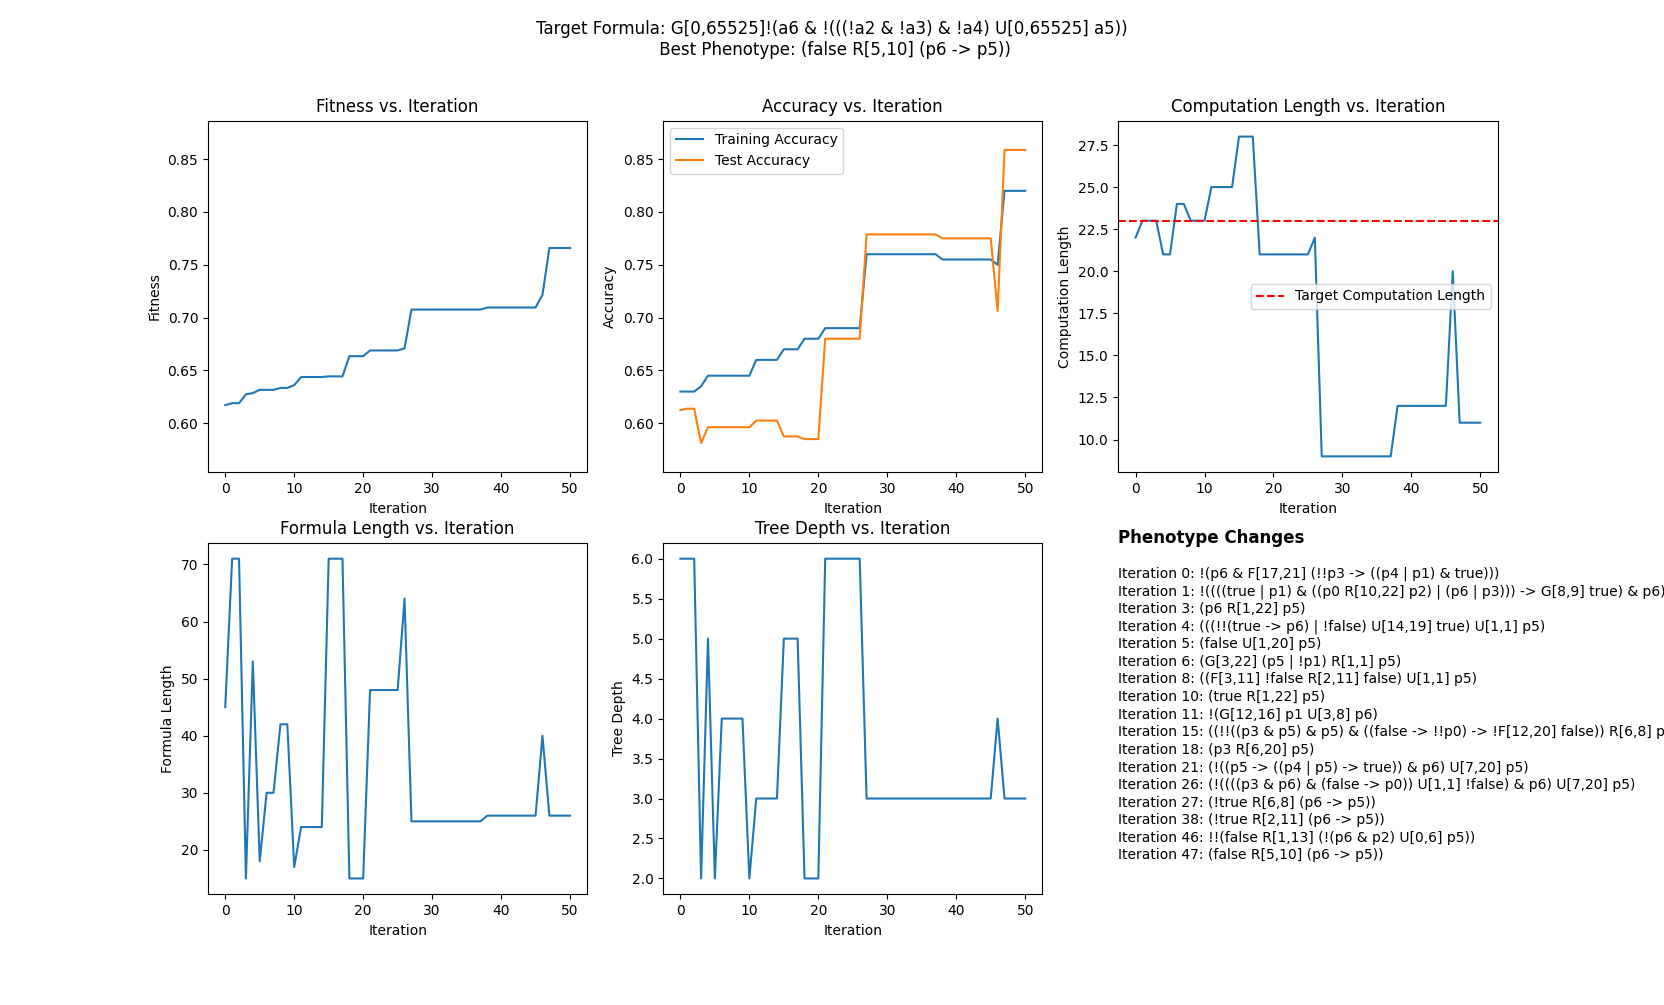
\includegraphics[width=1.1\textwidth]{figs/log_fmsd17_formula2.txt.png}
    \caption{Training plots of $DSGE^+$ formula 2 of the DragonEye UAS benchmark.}
    \label{fig:fmsd17_formula2}
\end{figure}

\begin{figure}
    \centering
    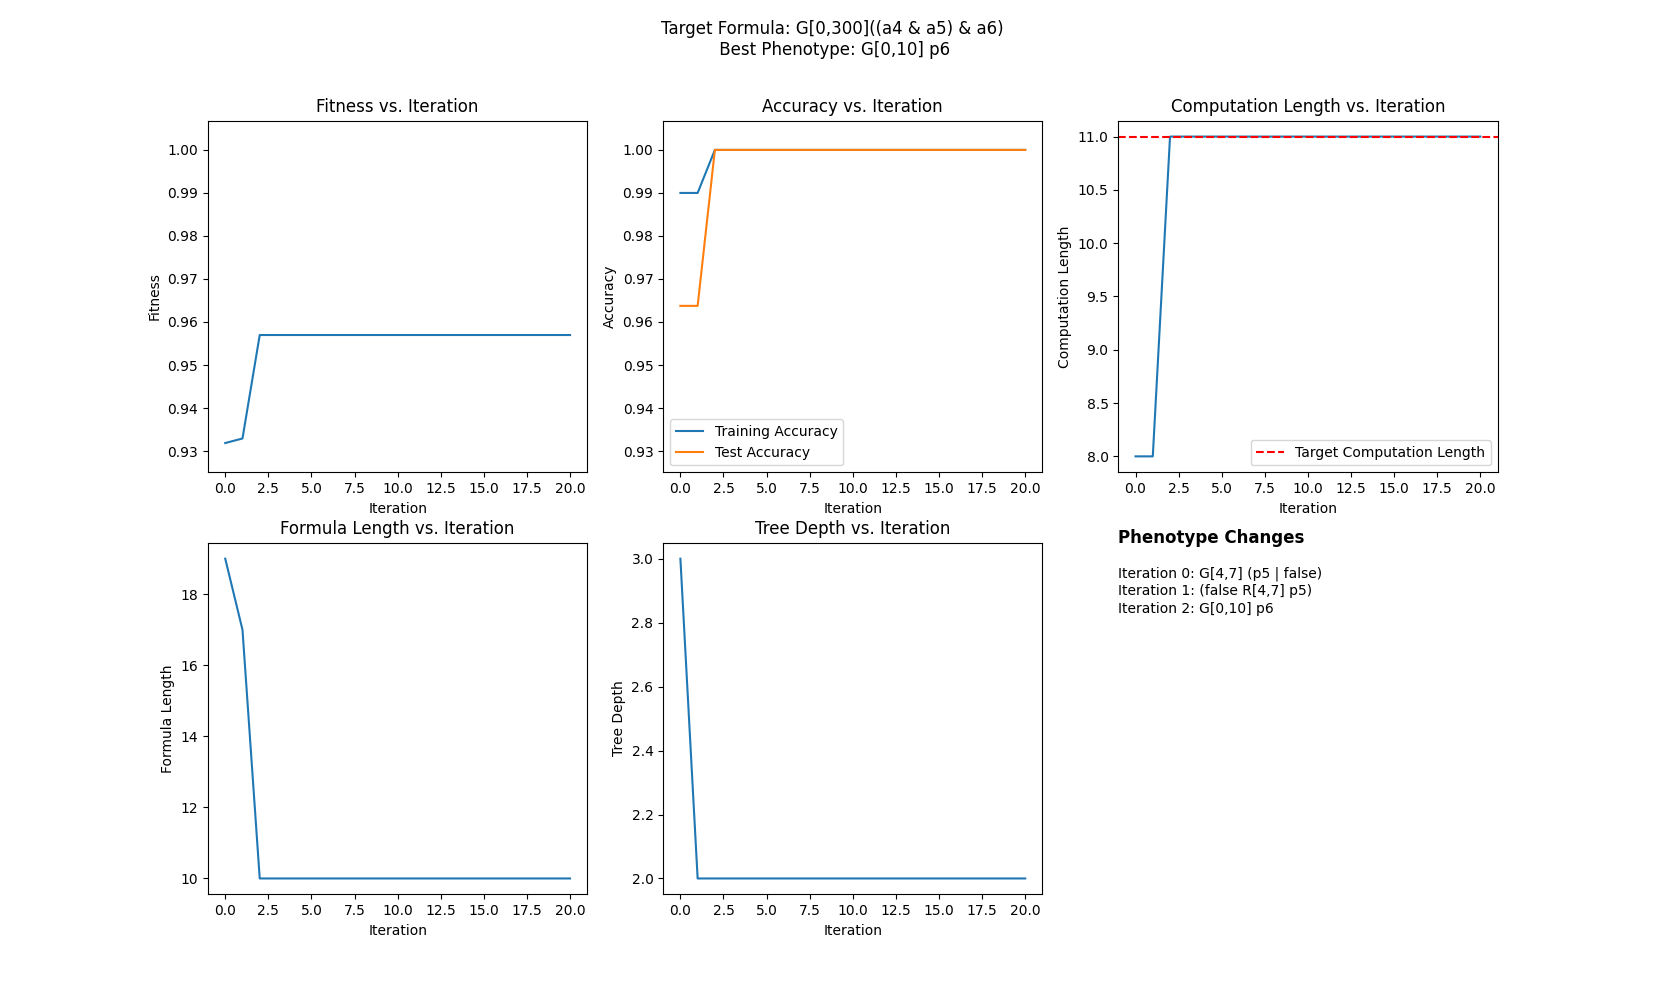
\includegraphics[width=1.1\textwidth]{figs/log_fmsd17_formula3.txt.png}
    \caption{Training plots of $DSGE^+$ formula 3 of the DragonEye UAS benchmark.}
    \label{fig:fmsd17_formula3}
\end{figure}

\begin{figure}
    \centering
    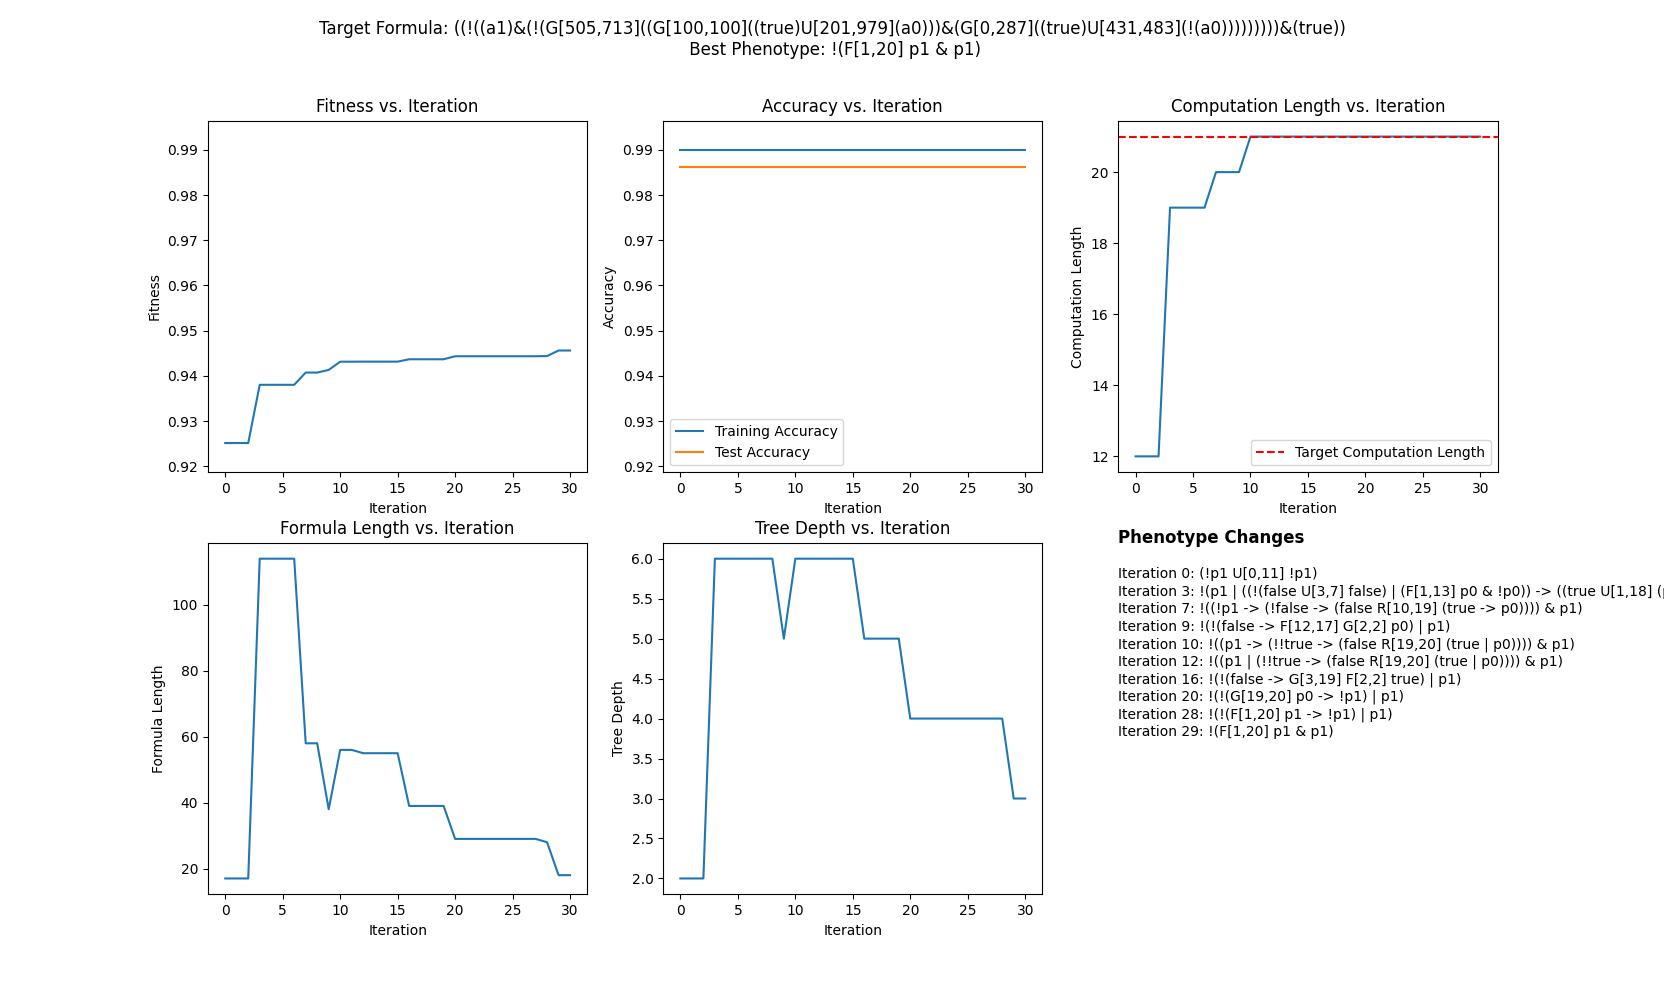
\includegraphics[width=1.1\textwidth]{figs/log_nasa-atc_formula1.txt.png}
    \caption{Training plots of $DSGE^+$ formula 1 of the NASA's NextGen Air Traffic Control benchmark.}
    \label{fig:nasa-atc_formula1}
\end{figure}

\begin{figure}
    \centering
    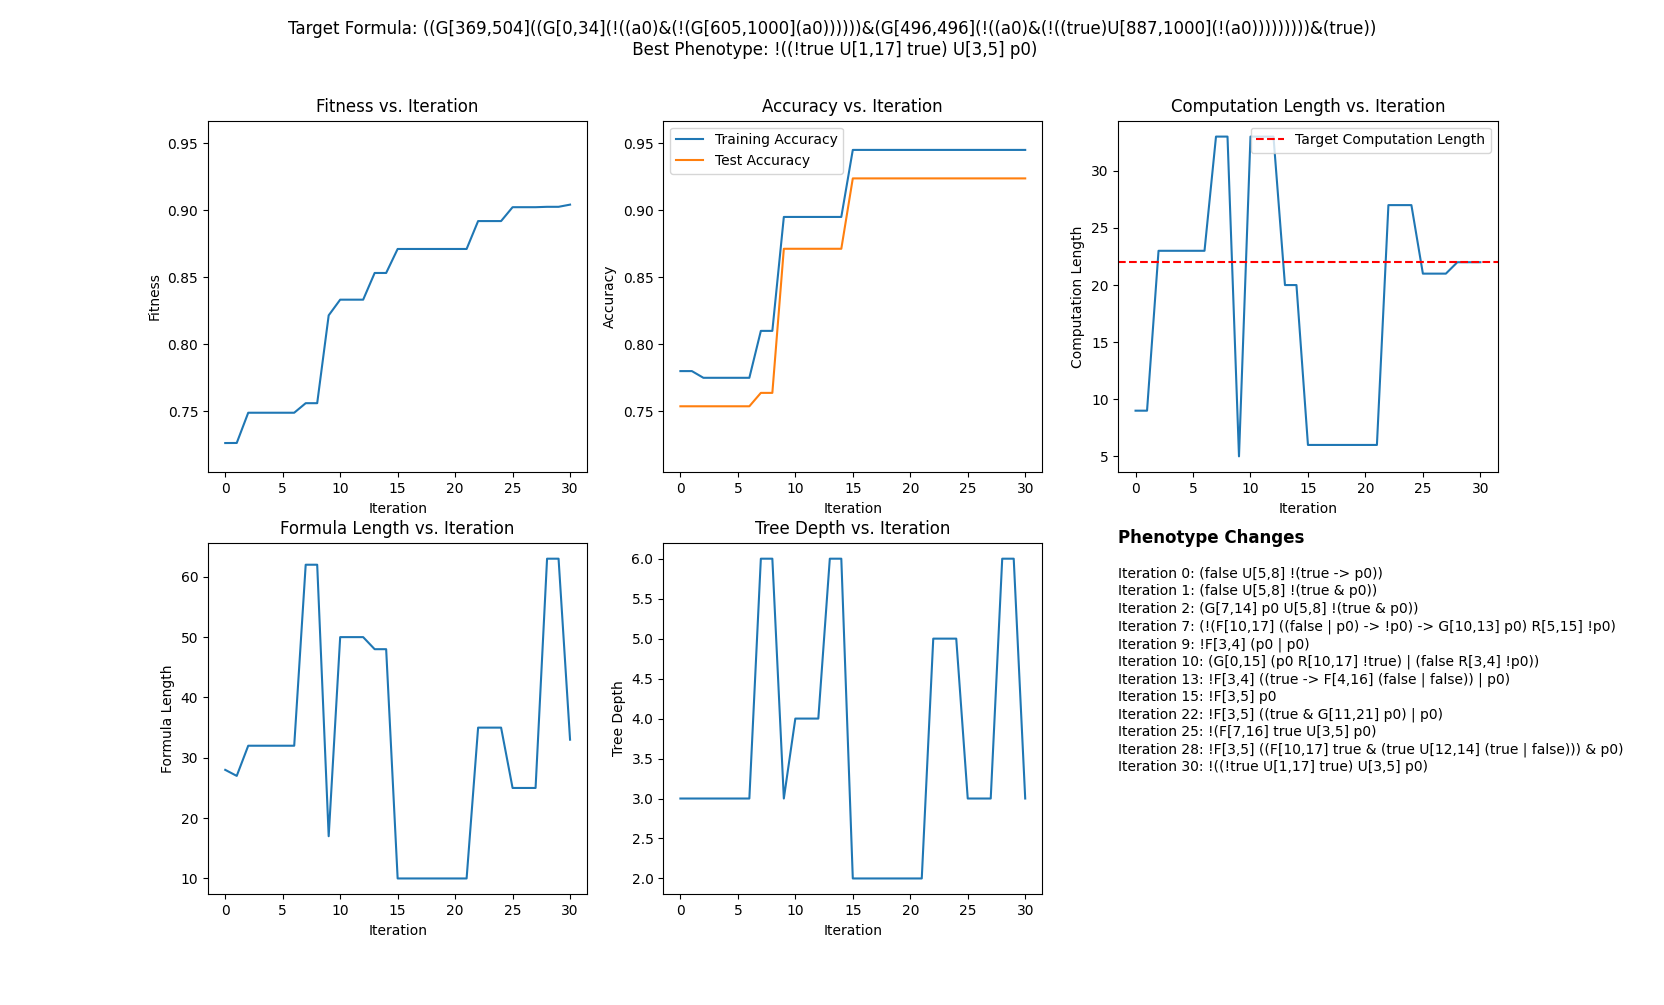
\includegraphics[width=1.1\textwidth]{figs/log_nasa-atc_formula2.txt.png}
    \caption{Training plots of $DSGE^+$ formula 2 of the NASA's NextGen Air Traffic Control benchmark.}
    \label{fig:nasa-atc_formula2}
\end{figure}

\newpage
\section{Conclusion and Future Work}
We have shown that MLTL is a strict subset of regular languages, and that the MLTL inference problem is well-defined.
We proposed a novel GE algorithm, DSGE$^+$, that combines the advantages of DSGE and SGE while addressing the initialization complexity and insufficient genotype length issues of DSGE.
We also proposed a set of MLTL benchmarks for future research, and reported and analyzed the performance of DSGE$^+$ on these benchmarks.

\subsubsection{Future work} includes proving theoretical learnability of MLTL from example traces. 
Relatively simply formulae, such as $p \mathcal{U}_[0, 10] q$, characterizes an exponential number of traces. 
Thus we hope to prove that some $(1+\epsilon)$ approximation of a set of traces $\Pi$ can be achieved by a formula of length logarithmic in $|\Pi|$. 
Possible works we can explore include the general Probably Approximately Correct (PAC) learning framework introduced by Valiant \cite{Valiant_PAC} in 1984, and the recent work by Perez et al. \cite{Perez_Somenzi_Trivedi_2023} on a PAC algorithm for learning LTL.

As discussed in our experimental evaluation section, the quality of the example traces $\Pi$ is crucial to GE. 
Thus we wish to explore the effects of different sampling strategies for generating $\Pi$ that gives better edge cases to distinguish between formulae such as $\mathcal{G}_[a, b] (p_0 \land p_1)$ and $\mathcal{G}_[a, b] p_0$.
One possible approach is to sample traces where each bit is $1$ with probability $p$ and $0$ with probability $1-p$, and ranging $p$ uniformly from $0$ to $1$. 
Another approach is to explore notions of formula branch coverage, posed by work stemming from the FPROGG tool (backslash cite Alek). 

As seen in our experimental evaluation, many formulae were learned throughout DSGE$^+$ that could be simplified to a more concise formula.
Thus we wish to explore the effects of applying a formula simplification operator to the population at each iteration.
For instance, Johannsen et al. \cite{Johannsen_Jones_Kempa_Rozier_Zhang_2023} integrates MLTL formula rewriting rules into the recently introduced C$2$PO extension for R$2$U$2$.

Additionally we wish to explore the effects of the genetic difference operator on the performance of DSGE$^+$. 
Specifically, we conjecture that applying a $k$-clustering selection strategy will improve the performance of DSGE$^+$ by maintaining population diversity while still selecting for high fitness individuals.

Lastly, we wish to perform a more thorough experimental evaluation of DSGE$^+$. One approach is to compare the performance of DSGE$^+$ against GE, SGE, and DSGE on the same set of benchmarks.
A more interesting approach would be to conduct a case study on a real-world application of MLTL inference, such as specification mining for formal verification, debugging systems, behavior classification, and formula reparation. 
One of the original motivations for applying GE to MLTL inference was to generate a population of interpretable MLTL formulae that could help a user repair an incorrectly specified MLTL formula.



%
% ---- Bibliography ----
%
% BibTeX users should specify bibliography style 'splncs04'.
% References will then be sorted and formatted in the correct style.
%
\newpage
\bibliographystyle{splncs04}
\bibliography{mybibliography}
%
\end{document}
